%
% This document is available under the Creative Commons Attribution-ShareAlike
% License; additional terms may apply. See
%   * http://creativecommons.org/licenses/by-sa/3.0/
%   * http://creativecommons.org/licenses/by-sa/3.0/legalcode
%
% Created: 2011-08-14 17:43:38+02:00
% Main authors:
%     - Jérôme Pouiller <jezz@sysmic.org>
%

\part{Gestion des évènements}

{
\setbeamertemplate{background canvas}{}
\begin{frame}[plain]
  \partpage
  \begin{textblock}{10}(6,11)
    %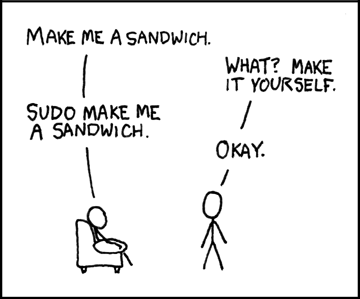
\includegraphics[height=30mm,width=30mm]{sandwich}
    \begin{quote}
      \rmfamily\textit\textbf\color{darkgray}{\large
        ``Q. How did the programmer die in the shower?\\
        A. He read the shampoo bottle instructions: Lather. Rinse. Repeat.''}
      %\vskip3mm\hspace*\fill{\small--- William Shakespeare, Hamlet}
    \end{quote}
  \end{textblock}
\end{frame}
}

\begin{frame}
  \tableofcontents
\end{frame}

\begin{frame}{Les OS monotâches}
  \begin{itemize}
  \item Permettent  surtout de fournir une  interface de programmation
    commune pour différents programmes ou drivers
  \item Le plus connu est sûrement MS-DOS
  \item Les OS génériques sont maintenant tous multitâches
  \item  Les  derniers  restant   se  trouvent  sur  des  applications
    spécialisés : Consoles de jeux, calculatrice, etc...
  \item Ils ont l'intérêt d'être simple à développer
  \end{itemize}
\end{frame}

\begin{frame}{Une définition}
  \begin{itemize}
  \item \textbf{Temps de réponse} : temps entre un évènement et la fin
    du traitement de l'évènement.
  \end{itemize}
\end{frame}

\section{Scrutation des évènements}
\begin{frame}[fragile]{Scrutation des évènements}
  \begin{itemize}
  \item Aussi appelé \emph{polling}
  \item Boucle infinie
  \item On teste des valeurs des entrées à chaque tour de boucle
  \end{itemize}
  \begin{lstlisting}
#define sensor1 *((char *) 0x1234)
#define sensor2 *((char *) 0xABCD)

int main() {
  while (1) {
    if (sensor1)
      action1();
    if (sensor2)
      action2();
  }
}
  \end{lstlisting}
\end{frame}

\begin{frame}{Scrutation}
  \begin{itemize}
  \item Temps de réponse au  évènements en pire cas facile à calculer:
    Pire temps pour parcourir la boucle
  \item Simple à programmer lorsqu'il  y a peu de périphériques (ayant
    des temps  de réaction  similaires). On peut  les scruter  en même
    temps
  \item Utilisation du CPU sous optimal. Beaucoup de temps est utilisé
    pour lire la valeur des  entrée. Ceci est particulièrement vrai si
    les évènements sont peu fréquents
  \item Si certains évènements entraînent des temps de traitement long
    ou si il y a beaucoup  d'entrées à scruter, le temps de réponse en
    pire cas peut rapidement devenir très grand
  \item Tous les évènements sont traités avec la même priorité
  \item  Mauvaise modularité  du code.  Ajouter des périphériques
    revient à repenser tout le système
  \end{itemize}
\end{frame}

\section{Gestion d'interruptions synchrones}

\begin{frame}{Interruptions synchrones}
  \begin{itemize}
  \item Appelé aussi Background/Foreground
  \item Gestion des évènements dans les interruptions
  \end{itemize}
  \begin{center}
    \pgfimage[width=6cm]{pics/model_bgfg}
  \end{center}
\end{frame}

\begin{frame}[fragile]{Interruptions synchrones}
  Concrètement:
  \begin{lstlisting}
#define PTR_DATA ((char *) 0x1234)

void isr() {
  action1(*PTR_DATA);
  *PTR_DEVICE_ACK = 1;
}

int main() {
  enable_interrupt(isr, 0x1);
  while(1) {
    ; // Optionnal background computing
  }
}
  \end{lstlisting}
\end{frame}

\begin{frame}{Interruptions synchrones}
  \begin{itemize}
  \item Temps de réponse au évènements plutôt bon
  \item Temps de réponse assez simple à calculer. Somme de
    \begin{itemize}
    \item Temps de traitement de l'évènement
    \item Temps de traitement des évènements de priorité supérieures
    \item Temps du changement de contexte (plus ou moins constant)
    \item Pire intervalle de temps ou les interruptions sont désactivées
    \end{itemize}
  \item[$\rightarrow$] Dans  un système simple, ça peut  se calculer à
    la louche
  \item Le  temps de réponse en pire  cas des calculs en  tâche de fond
    est quasiment  identique au traitement  par scrutation (attention
    tout de même à la fréquence maximum des interruptions)
  \end{itemize}
\end{frame}

\begin{frame}{Qu'est-ce qu'une interruption?}
  Il existe trois type d'interruptions:
  \begin{itemize}
  \item Les interruptions matérielles:
    \begin{itemize}
    \item   \textbf{IRQ}   (aussi   appelé   Interruption   externe).
      Asynchrone.   Exemples:  clavier,   horloge,  bus,  DMA,  second
      processeur, etc...
    \item  \textbf{Exception}.   Asynchrone  ou Synchrone.   Exemples:
      Division  par zéro,  Erreur arithmétique,  Erreur d'instruction,
      Erreur d'alignement, Erreur de page, Breakpoint matériel, Double
      faute,  etc...

      \note{Un  overflow arithmétique ne  produit pas  d'exception, il
        lève le flags ``retenue''\\}

      \note{Un  breakpoint  logiciel change  une  instruction par  une
        interruption  logicielle. Un  break point  software  n'est pas
        possible en ROM alors que le breakpoint hardware oui\\}
    \end{itemize}
  \item \textbf{Logicielle}. Déclenchée par une instruction. Synchrone.
  \end{itemize}
\end{frame}

\begin{frame}{Fonctionnement d'une interruption}
  \begin{center}
    \pgfimage[width=10cm]{pics/interuption-1}
  \end{center}
\end{frame}

\begin{frame}{Fonctionnement d'une interruption}
  Quand une  interruption est levée:
  \begin{itemize}
  \item le CPU sauve en  partie ou en totalité le contexte d'exécution
    (principalement le pointeur d'instruction) sur la pile
  \item Le CPU passe en mode superviseur (nous y reviendrons)
  \item  Le CPU  recherche dans  l'IVT (\emph{Interrupt  Vector Table}
    aussi  appelée  IDT,  \emph{Interrupt  Description  Table})  l'ISR
    (\emph{Interruption Service Routine}) associée
  \item Le CPU place le pointeur d'instruction sur l'ISR
  \item  L'ISR traite  l'évènement (fin  de traitement  d'une E/S,
    etc...)
  \item L'ISR acquitte la  réception de l'interruption indiquant qu'une
    nouvelle  donnée peut-être  traitée.
  \item L'ISR restaure le (un) contexte
  \end{itemize}
\end{frame}

\begin{frame}{Fonctionnement d'un PIC}
  Le PIC (Programmable Interrupt Controller) est un composant matériel
  permettant  la gestion  des  IRQ.  Il peut-être  intégré  au CPU  ou
  externe (ou à cheval entre les deux...). Il permet en particulier:
  \begin{itemize}
  \item Activer ou de désactiver des IRQ
  \item De masquer temporairement une IRQ
  \item De mettre en queue une interruption temporairement masquée
  \item De contrôler la priorité des interruptions
  \end{itemize}
  Il arrive fréquemment  qu'un PIC soit multiplexé sur  une seule ligne
  d'IRQ. Dans  ce cas, le premier  étage d'ISR lit un  registre du PIC
  pour connaître  le numéro de l'IRQ.   (Cas notoire du  8259A sur les
  architectures x86)

  \note {Il existe aussi des APIC (Advanced PIC). Sur PC notamment}
\end{frame}

\begin{frame}{Exemple}
  Exemple classique d'intégration d'un PIC multiplexé sur une IRQ:
  \begin{center}
    \pgfimage[width=10cm]{pics/interuption-3}
  \end{center}
\end{frame}

\begin{frame}{Exemple}
  \begin{enumerate}
  \item Le périphérique \emph{Timer} lève sa ligne d'IRQ
  \item Le PIC reçoit l'interruption et lève une IRQ du processeur
  \item  Le processeur  complète  l'instruction courante  et sauve  le
    registre d'instruction (PC) et le registre d'état (PSW)
  \item La tâche courante devient interrompue (Nous y reviendrons)
  \item Le premier étage d'ISR est appelé
  \item  Le  gestionnaire d'interruption  complète  la sauvegarde  des
    registres
  \item   Le  gestionnaire  d'interruption   demande  au   PIC  quelle
    interruption à  été appelée  et il lit  dans l'IVT quelle  ISR est
    associée
  \end{enumerate}
\end{frame}

\begin{frame}{Exemple}
  \begin{enumerate}
    \setcounter{enumi}{7}
  \item Le  gestionnaire d'interruption se branche  sur l'ISR associée
    (ici, ISR1)
  \item L'IRQ du processeur est acquittée. Les autre IRQ peuvent ainsi
    être levées
  \item  L'ISR1 lit la  valeur provenant  du \emph{Timer}  et acquitte
    l'interruption  du \emph{Timer}. Ce  périphérique peut  de nouveau
    lever des IRQ.
  \item Les registres généraux sont restaurés
  \item Le contexte d'exécution est restauré
  \item Le registre PC est restauré
  \end{enumerate}
\end{frame}

\subsection{Utilisation des interruptions}

\begin{frame}{Exemple}
  Exemple de différence d'approche entre la gestion par scrutation et
  la gestion par interruption:\\

  Prenons  l'acquisition  de   donnée  à  partir  d'un  convertisseur
  analogique/numérique asynchrone
  \begin{itemize}
  \item  Dans  le  cas  du  traitement  par  scrutation,  nous  allons
    périodiquement voir  si un résultat est arrivé.  Beaucoup de temps
    est  consommé  pour  rien   et  lorsque  le  résultat  arrive,  le
    traitement du résultat sera retardé
  \item  Une interruption  est  levée quand  une  nouvelle donnée  est
    disponible. Le processeur peut alors la traiter.
  \end{itemize}
\end{frame}

\begin{frame}{Latence des interruptions}
  \begin{itemize}
  \item Un périphérique ne génère pas d'IRQ si la précédente n'est pas
    acquittée (en principe)
  \item Vu  que les  interruptions sont souvent  multiplexées, les
    interruptions sont  souvent désactivées lors de  la première phase
    de traitement
  \item  Pour des  raisons techniques,  il est  parfois  nécessaire de
    désactiver les interruptions
  \item  Le partage  de l'information  entre les  interruptions  et le
    reste   du   programme  nécessite   parfois   de  désactiver   les
    interruptions (Nous y reviendrons)
  \end{itemize}
  Les conséquences:
  \begin{itemize}
  \item Augmente les temps de réponses
  \item Temps réponse plus difficile à calculer
  \item  Risque   de  perdre  des  interruptions  (Dans   ce  cas,  une
    interruption \emph{overrun} est (devrait être) déclenchée)
  \end{itemize}
\end{frame}

\begin{frame}{Précautions avec les interruption}
  \begin{itemize}
  \item Acquitter l'interruption le plus tôt possible
  \item Rester le moins de temps possible dans une interruption
  \item Accéder à un minimum de données pour éviter d'avoir à partager
    des données avec le background
  \item Transférer un maximum de traitement hors de l'interruption
  \item[$\rightarrow$] Gestion des interruptions asynchrones
  \end{itemize}
\end{frame}

\section{Gestion d'interruptions asynchrones}

\begin{frame}[fragile]{Interruptions asynchrones}
  \begin{itemize}
  \item  Interruption  séparée en  deux  parties:  \emph{top half}  et
    \emph{bottom half}
  \item On délègue le maximum de traitement au \emph{bottom half}
  \item Permet de décharger les interruptions
  \item Permet  de plus facilement prendre en  compte des interactions
    entre  les   évènements  (exemple,  possibilité   d'attendre  deux
    évènements avant d'effectuer une action)
  \end{itemize}
\end{frame}

\begin{frame}[fragile]{Interruptions asynchrones}
  \begin{lstlisting}
#define PTR_DATA ((char *) 0x1234)

int gotit = 0;
void isr() {
    gotit++;
    *PTR_DEVICE_ACK = 1;
}

int main() {
  enable_interrupt(isr, 0x1);
  while(1) {
     if (gotit) {
       gotit--;
       action1();
     }
  // Optionnal background computing
  }
}
  \end{lstlisting}
  \note{Il y a un bug à cause  du partage de gotit, mais on en parlera
    plus tard}
\end{frame}

\section{Protection des structures de données}

\begin{frame}[fragile]{Exemple de partage de données}
  Imaginons le code suivant:
  \begin{lstlisting}
#define PTR_DATA ((char *) 0x1234)
int a = 0;
char t[255];
void isr() {
  t[a++] = *PTR_DATA;
  *PTR_DEVICE_ACK = 1;
}
void main() {
  enable_interrupt(isr, 0x1);
  while(1) {
    if (a)
      action1(t[--a]);
    // Optionnal background computing
  }
}
  \end{lstlisting}
\end{frame}

\begin{frame}[fragile]{Exemple de partage de données}
  Prenons le  cas où  \verb+f+ traite l'interruption  précédente (donc
  \verb+a = 1+) et qu'une nouvelle interruption est déclenchée:
  \begin{columns}
    \begin{column}{5cm}
      \begin{lstlisting}[showlines=true,emptylines=10]
--a; // a = 0;





action1(t[a]);
// Lecture de t[1] au lieu de t[0]!
       \end{lstlisting}
     \end{column}
     \begin{column}{5cm}
      \begin{lstlisting}[showlines=true,emptylines=10,escapeinside=\{\}]

t[a] = *PTR_DATA;
// t[0] est {é}cras{é}!
a++;
// a = 1 maintenant
*PTR_DEVICE_ACK = 1;


       \end{lstlisting}
    \end{column}
  \end{columns}
  Au lieu de lire correctement  la première valeur retournée par l'ISR
  puis la seconde, nous lirons  tout d'abord une valeur aléatoire puis
  la valeur retournée par la seconde interruption.
\end{frame}

\begin{frame}{Comment éviter le problème?}
  Les problèmes d'accès concurrents se traduisent très souvent par des
  \emph{races  conditions}.   C'est à  dire  des problèmes  aléatoires
  produit par une séquence particulière d'évènements
  \begin{itemize}
  \item   Les  \emph{races  conditions}   sont  souvent   difficiles  à
    reproduire et à identifier
  \item Les  \emph{races conditions} peuvent être latente  dans le code
    et se déclarer suite à une modification de l'environnement externe
  \item Une race condition coûte chère (difficulté de correction, peut
    potentiellement atterrir en production)
  \end{itemize}
  Comment s'en protéger?
  \begin{itemize}
  \item  Ne  pas  partager de données avec les interruptions
  \item Utiliser des accès atomiques
  \item  Utiliser  des  structures  adaptées: buffers  circulaires  et
    queues
  \item  Désactiver  les  interruptions  lors  d'accès  à  des  données
    partagées
  \end{itemize}
\end{frame}

\subsection{Buffer circulaire}

\begin{frame}[fragile]{Buffer circulaire}
  \begin{lstlisting}
char buf[SIZE];
void init() {
  w = r = 0;
}
void write(char c) {
  if ((w + 1) % SIZE == r )
    ; //buffer is full
  buf[w] = c;
  w = (w + 1) % SIZE;
}
void read() {
  if (w == r)
    ; //buffer is empty
  ret = buf[r];
  r = (r + 1) % SIZE;
}
  \end{lstlisting}
\end{frame}

\subsection{Queue}

\begin{frame}{Queue}
  Même fonctionnement  que le buffer circulaire, mais  avec un tableau
  de structure.

  Il est aussi possible de  faire des \emph{queue} d'objets de tailles
  différentes.  Dans  ce cas, faire très attention  à l'allocation des
  objets.   L'allocation  dynamique est  rarement  une opération  très
  bornée  dans  le temps  et  doit  être  utilisée avec  précaution  à
  l'intérieur des interruptions et des tâches temps réelles.
\end{frame}

\subsection{Désactivation des interruptions}

\begin{frame}{Désactivation des interruptions}
  Si l'utilisation de Buffer circulaires ne résout pas le problème, il
  est possible de désactiver les interruptions.

  La désactivation des interruptions peut entraîner des latences dans la
  gestion  des  interruptions  et  des  pertes  d'interruptions  le  cas
  échéant.
\end{frame}

\begin{frame}{Cas des interruption en milieu multicoeurs}
  \begin{itemize}
  \item  On ne  désactive que  les interruptions  locales (sur  le CPU
    courant)
  \item Une interruption peut se produire sur un autre coeur
  \item Nécessité d'utiliser un mécanisme supplémentaire d'exclusion
  \item \emph{Spin lock} souvent utilisé pour ce cas.
  \item  Pas beaucoup  d'autres  choix.  Par  conséquent les  sections
    critiques dans les interruptions doivent être très limitées
  \end{itemize}
\end{frame}

\subsection{Spin Lock}

\begin{frame}[fragile]{Spin Lock}
  Attente active.\\
  Nécessite une instruction assembleur  permettant un accès en lecture
  et une écriture  en une instruction: \\
  \texttt{test\_and\_set} affecte le registre d'état en fonction de la
  valeur  du registre  et affecte  la valeur  1 au  registre.
  \begin{lstlisting}
void lock(int m) {
  while(atomic_test_and_set(m))
     ;
}

void unlock(int m) {
  m = 0;
}
  \end{lstlisting}
\end{frame}

\section{Les limites du monotâche}

\begin{frame}{Problèmes de la gestion des interruptions asynchrones}
  Nous n'avons pas résolu notre problème récurent:
  \begin{itemize}
  \item  Le partage  de l'information  entre les  interruptions  et la
    boucle principale entraîne des latences
  \end{itemize}
  On retrouve certains problèmes que l'on avait avec la scrutation:
  \begin{itemize}
  \item  Ne permet  pas de  prioriser  les traitements  dans la  boucle
    principale
  \item Interaction entre les évènements complexe
  \end{itemize}
  \note{Parler du mot clef volatile\\}
  \note{Montrer ici  le code du HC08  de la Cobalt.  Commencer par une
    description du but,  du hard: 3 ADC pour  Joystick, deux encodeur,
    clavier matricé,  bus can, prise coaxiale, 20ms,  sytème pour deux
    Cobalt   sur   un  même   réseau   montrer  doc/cobalt/schema   de
    principe.pdf.   Montrer MC68HC908GZ16.h  (montrer  les registres),
    MC68HC908GZ16.c   (montrer   volatile),   link.prm  (montrer   les
    vecteurs),   start.c  (copie  ROM   vers  RAM),   interrupt.c  (en
    particulier intGenlock), main.c (fonction loop)\\}
\end{frame}


\section{Le temps partagé}

\begin{frame}{Concurrence}
  \begin{itemize}
  \item   Des   tâches   concurrentes   sont   des   tâches   exécutées
    séquentiellement sur un seul processeur en entrelaçant l'exécution
    de chaque tâches
  \item  Pour les tâches,  le temps  partagé est  transparent.  Chaque
    tâche à l'impression d'avoir le CPU pour elle-seule
  \item  On  trouvera aussi  le  terme  de  \emph{multitâches} ou  de
    \emph{temps partagé}
  \end{itemize}
\end{frame}

\begin{frame}{Concurence}
   La programmation concurrente N'EST  PAS de la programmation parallèle
  (même les système multicoeurs sont souvent concurrent et parallèle):
  \begin{center}
    \pgfimage[width=10cm]{pics/concurentVsParallel}
  \end{center}
\end{frame}

\begin{frame}[fragile]{Programmation multitâche}
\begin{lstlisting}
#include <unistd.h>

int main() {
  int r;

  r = fork();
  if (r < 0) {
     // Error
  } else if (r > 0) {
    // Parent
  } else /* r == 0 */ {
    // Child
  }
}
\end{lstlisting}
\end{frame}

\begin{frame}{Concurrence}
  Migration d'un système avec gestion asynchrone des interruptions vers
  un système multitâches:
  \begin{center}
    \pgfimage[width=10cm]{pics/model_multitask}
  \end{center}
\end{frame}

\begin{frame}{Tâches concurrentes}
  Pour les  systèmes plus complexes ou pour  facilité la réutilisation,
  un   système   multitâche   est   plus   approprié   qu'un   système
  \emph{Foreground/Background}.
  \begin{itemize}
  \item Facilite la gestion des évènements
  \item Permet de prioriser les traitements
  \end{itemize}
  \note{Parler  des différentes  états des  tâches ici.  Il  manque un
    slide avec du code.}
\end{frame}

\begin{frame}{Etats des tâches}
  \begin{center}
    \input{pics/task_states}
  \end{center}
\end{frame}


\subsection{Changement de contexte}

\begin{frame}{Le changement de contexte}
  Chaque tâche possède une pile en mémoire. Une liste globale contient:
  \note{Faire un schéma}
  \begin{itemize}
  \item les états de toutes les tâches
  \item l'emplacement de la pile en mémoire
  \item le contexte d'exécution, c'est-à-dire une sauvegarde des registres
  \end{itemize}
  Lors du changement de contexte
  \begin{itemize}
  \item  on  sauvegarde  le   contexte  de  la  tâche  précédente,  en
    particulier son pointeur de pile et son pointeur d'instruction
  \item on restaure le contexte de la nouvelle tâche
  \item on restaure le pointeur d'instruction
  \end{itemize}
  Dans la  pratique, il y a  des petites subtilités  dépendantes de la
  manière dont le changement de contexte à été amené.
\end{frame}

\begin{frame}{Le changement de contexte}
  \begin{center}
    \pgfimage[width=7cm]{pics/context_switch}
  \end{center}
\end{frame}

\begin{frame}{Multitâche non-préemptif}
  Le changement de contexte  peut-être volontaire par les tâches. Dans
  ce   cas,  la   tâche   ayant  terminé   son  traitement   appellera
  explicitement   la  fonction   \emph{schedule}   qui  effectuera   la
  changement  de   contexte.  le  système  est   dit  non-péemptif  ou
  multitâche collaboratif.
\end{frame}

\begin{frame}{Multitâche non-préemptif}
  Ce type  de système implique une  latence difficilement quantifiable
  entre un évènement et sont traitement:
  \begin{center}
    \pgfimage[width=7cm]{pics/preemptive-no}
  \end{center}
\end{frame}

\begin{frame}{Multitâche non-préemptif}
  \begin{enumerate}
  \item  Une tâche  non prioritaire  est en  cours d'exécution  et est
    interrompue par un évènement (une IRQ)
  \item L'ISR est appellé
  \item Le traitement  l'IRQ rend une tâche de  haute priorité prête à
    être exécutée
  \item  A  la fin  de  l'ISR,  le système  rend  le  CPU  à la  tâche
    non-prioritaire
  \item Quand  la tâche non-prioritaire termine  sont traitement, elle
    appelle \texttt{schedule}
  \item L'ordonnanceur donne la main à la tâche de forte priorité
  \item La tâche de haute priorité peut (enfin) s'exécuter
  \end{enumerate}
\end{frame}

\begin{frame}{Multitâche préemptif}
  Un  système  multitâche préemptif  va  être  capable  de changer  de
  contexte lors des interruptions:
  \begin{center}
    \pgfimage[width=10cm]{pics/preemptive-yes}
  \end{center}
\end{frame}

\begin{frame}{Multitâche préemptif}
  \begin{enumerate}
  \item  Une tâche  non prioritaire  est en  cours d'exécution  et est
    interrompue par un évènement (une IRQ)
  \item L'ISR est appelée
  \item Le traitement  l'IRQ rend une tâche de  haute priorité prête à
    être exécutée
  \item A la fin de l'ISR, le système appel le scheduler
  \item Le scheduler donne la main a la tâche de haute priorité
  \item  Quand  la tâche  prioritaire  termine  sont traitement,  elle
    appelle \texttt{schedule}
  \item   Vu  qu'il  n'y   a  plus   tâche  prioritaire   à  exécuter,
    l'ordonnanceur redonne la main à la tâche de faible priorité
  \end{enumerate}
\end{frame}

\begin{frame}{Le changement de contexte sur interruption}
  \begin{center}
    \pgfimage[width=10cm]{pics/interuption-2}
  \end{center}
\end{frame}

\begin{frame}[fragile]{Round robin}
  Examinons  le cas de  deux tâches  de priorité  égales n'effectuant
  jamais de relanchement volontaire:
  \begin{lstlisting}
task1() {
  for(;;) ;
}
task2() {
  for(;;) ;
}
  \end{lstlisting}
\end{frame}

\begin{frame}[fragile]{Round robin}
  Dans ce cas, si aucune interruption ne se produit, la première tâche
  à avoir pris la main ne la rendra jamais. Afin de reprendre la main,
  on  utilise une  interruption  d'horloge.  Celle-ci  garanti que  le
  système  pourra périodiquement  reordonnancer les  tâches.  La période
  l'horloge utilisée est appelée quantum de temps ou HZ dans le cas de
  Linux.

  Dans   ce  cas-ci,   l'ordonnanceur  devra   donner  une   période  à
  \emph{task1} puis une période à  \emph{task2} et ainsi de suite.  Ce
  comportement s'appelle \emph{Round-Robin} ou \emph{Tourniquet}.
  \begin{center}
    \input{pics/round_robin}
  \end{center}
\end{frame}



% \section{Biographie}

% \begin{frame}{Biographie}
%   \begin{itemize}
%   \item G. Bois, M. De Nanclas, L. Filion, \emph{Real time systems concepts}, Ecole Polytechnique de Montréal
%   \item VxWorks, \emph{VxWorks Programers Guide V5.5}
%   \item Wikipedia: PIC, APIC, Interrupts
%   \end{itemize}
% \end{frame}
